%%% Research Diary - Entry
%%% Template by Mikhail Klassen, April 2013
%%% 
\documentclass[11pt,letterpaper]{article}
\newcommand{\workingDate}{\textsc{2018 $|$ June}}
\newcommand{\userName}{Carter Rhea}
\newcommand{\institution}{Universite de Montreal}
\usepackage{python}

\usepackage[]{algorithm2e}

\usepackage{listings}
\usepackage{color}
\definecolor{dkgreen}{rgb}{0,0.6,0}
\definecolor{gray}{rgb}{0.5,0.5,0.5}
\definecolor{mauve}{rgb}{0.58,0,0.82}
\usepackage{hyperref}
\hypersetup{
	colorlinks=true,
	linkcolor=blue,
	filecolor=magenta,      
	urlcolor=cyan,
}
\lstset{frame=tb,
	language=Java,
	aboveskip=3mm,
	belowskip=3mm,
	showstringspaces=false,
	columns=flexible,
	basicstyle={\small\ttfamily},
	numbers=none,
	numberstyle=\tiny\color{gray},
	keywordstyle=\color{blue},
	commentstyle=\color{dkgreen},
	stringstyle=\color{mauve},
	breaklines=true,
	breakatwhitespace=true,
	tabsize=3
}
\usepackage{researchdiary_png}
% To add your univeristy logo to the upper right, simply
% upload a file named "logo.png" using the files menu above.

\begin{document}
\univlogo

\title{Documentation for WVT}

%\begin{python}%
%print r"Hello \LaTeX!"
%\end{python}%
\textit{Documentation for my Weighted Voronoi Tessellations Algorithm.}

\tableofcontents

\newpage


\newpage
\section{Weighted Voronoi Tessellations}

\subsection{Introduction}
Before delving into Weighted Voronoi Tessellations, I would first like to simply describe why we care about them (other than the fact that they are pretty cool). In a few words: WVT allows for a binning scheme that is unbiased when compared with Voronoi Tessellations, Centroidal Voronoi Tesselations, or other binning methods. Once we have the WVT bins in place, we can use that information to general temperature maps for X-ray data (That's what I am interested in).

See \cite{Copin2018}, \cite{Diehl2008}, and \cite{Sanders2018} for more information.
\subsection{Signal-to-Noise}
For our particular application in X-ray astronomy, we are going to be interested in a signal-to-noise ratio dominated by count rates. Count Rates are a relatively easy quantity for us to compute. We use the following bash commands to calculate the \textbf{FLUX} at a pixel (This is assuming you skipped ahead and did all of the preprocessing as discussed in section 2!!).
\begin{lstlisting}
	punlearn eff2evt
	pset eff2evt clobber=yes
	eff2evt "input.fits" "output.fits"
\end{lstlisting}
%In order to get the count rate approximation we multiply the flux by the \textbf{Total\_Time\_Observation}.

The following equation are for pixel number $k$.
\begin{equation}\label{eqn:signal}
	Signal_k = Flux_k = \frac{C_k}{E_k \tau}-B_k
\end{equation}
\begin{equation}\label{eqn:noise}
	Noise_k = \sigma^2_k = \frac{C_k}{E^2_k\tau^2}+\sigma^2_{B_k}
\end{equation}

\begin{center}
	\begin{tabular}{|c|c|}
		\hline 
		Parameter & Definition \\
		\hline
		\hline
		$C_k$ & Raw Counts \\
		\hline 
		$E_k$ & Effective Area \\
		\hline 
		$\tau$ & Exposure Time \\
		\hline
		$B_k$ & Background Flux \\
		\hline 
		$\sigma_{B_k}$ & Uncertainty in Background Flux \\
		\hline
	\end{tabular}
\end{center}

\textbf{HOWEVER}, since we have done all of that wonderful data analysis described above, we have taken into account the Effective Area and Background Flux! Therefore our Signal-to-Noise calculation is reduced to the following simple expression:
\begin{equation}\label{eqn:S-N}
	Signal\-To\-Noise_k = \sqrt{Flux_k}
\end{equation}

This calculation and data-gathering occurs in the \textsc{read\_in} subroutine. 

That sums up signal-to-noise calculations in the current version of the code.

\subsection{Algorithm Run-Down}
This section will contain the pseudo-algorithm of my python code.

Before we are able to begin our algorithm (WVT) in earnest, we must have a decent initial guess! 

Enter \textbf{Bin Accretion}....
\subsubsection{Bin Accretion}
\begin{algorithm}[H]\label{algo:BA}
	\caption{Bin Accretion Algorithm}
	\KwData{Pixels}
	\KwResult{Initial Guess for WVT}
	initialization\;
	\While{Pixels left to be assigned}{
		\While{Criteria not all met}{
			Calculate pixel closest to bin centroid\;
			Calculate Adjacency\;
			Calculate Roundness\;
			Calculate Potential Signal-to-Noise\;
			\eIf{Criteria all met}{
				Add pixel to Bin\;
			}{
				Start new bin\;
			}
			\If{Signal-to-Noise too low}{
				Mark pixels unassigned\;
			}		
		}
	}
	Reassign all unassigned pixels to nearest bin\;
\end{algorithm}

With that out of the way we can discuss how I actually calculated the three different criteria: Adjacency, Roundness, Potential Signal-to-Noise.

\begin{itemize}
	\item Adjaceny: This one is simple: just check if the pixels are neighbors!
	\item Roundness: Ok so now we finally need to calculate some stuff... More explicity $R_{equiv}$ and $R_{max}$. $R_{max}$ is the maximum distance from the centroid for ALL pixels in bin. $R_{equiv}$ is a wonderfully horrendous quantity which is "the radius of a disk around the bin". Lets do a quick little derivation...
	\begin{equation}
		Area_{circle} = \pi r_{circle}^2 == n\pi\frac{d_{pix}}{2}^^2 = Area_{bin}
	\end{equation} 
	Solving for $r_{circle}$ we get,
	\begin{equation}
		r_{circle} = \sqrt{\frac{n}{\pi}} \ d
	\end{equation}
	And now we can calculate the roundness parameter which describes the compactness of the bin:
	\begin{equation}
		Roundness = \frac{R_{max}}{R_{equiv}} - 1
	\end{equation}
	We generally shoot for a value of $Roundness = 0.3$.
	\item Potential Signal-to-Noise: We add the pixel to the bin and then recompute the Signal-to-Noise. This needs to be less than the target Signal-to-Noise.
\end{itemize}

And now to the main event (which is not very much coding wise compared to bin accretion).

\subsubsection{WVT}
\begin{algorithm}[H]\label{algo:BA}
	\caption{Weighted Voronoi Tessellation Algorithm}
	\KwData{Bins}
	\KwResult{WVT Data}
	initialization $-->$ read in Bin Accretion Data\;
	\While{Bins not converged}{
		\For{bin in Bins}{
		Recalculate Signal-to-Noise\;
		Calculate Area\;
		Calculate Centroid\;
		Calculate Scale Length\;
		}
		Reassign Pixel to Closest Bin\;
	}
\end{algorithm}
And again we need to define two properties: Area and Scale Length.
\begin{itemize}
	\item Area: Area of bin. This is basically just the area of the pixels in the bin...
	\begin{equation}
		A_{bin} = (Pixel\_Length)^2*N_{pixels} 
	\end{equation}
	\item Scale Length: This scale length is the KEY to the WEIGHTED part of WVT.
	\begin{equation}
		\sqrt{\frac{A_{bin}}{\pi}\frac{S/N}{(S/N)_{target}}}
	\end{equation}
\end{itemize}

And really thats it!

\newpage


\section{Preprocessing of Data}
I finally decided to put this section as the second chapter since the main goal of this document is to outline the WVT algorithm. However, I also wanted to include this information for anyone interested in X-ray data reduction from \textit{CHANDRA}.

\subsection{Download Data}
Before we can begin to preprocess the data, we obviously need to have the data. Thankfully, this is incredibly simple! After downloading the data from the chandra website or using $$download\_chandra\_obsid \ \#OBSID $$ 
There exists a considerable amount of documentation on each file downloaded at 
$$\href{http://cxc.harvard.edu/ciao/threads/intro_data/}{http://cxc.harvard.edu/ciao/threads/intro\_data/} $$
\subsection{Reduce Data}
We reduced the data with the following command: $$chandra\_repro $$. For details on what the reprocessing does visit the following website:
$$\href{http://cxc.harvard.edu/ciao/ahelp/chandra_repro.html}{http://cxc.harvard.edu/ciao/ahelp/chandra\_repro.html}$$



\subsection{Region of Interest}
Once we have the reduction completed (which it is easily done using either of these algorithms...) we can move onto dealing with the data we are interested in...
We are assuming that you have already done the following  to create a region of interest:
\begin{itemize}
	\item opened ds9 and picked the region of interest: "ds9 ...evt2.fits \&" and RofI is called "simple.reg"
	\item Also created background image "simple\_bkgd.reg"
\end{itemize}

I saved them as physical units

Running this will create several files: PI, ARF, RMA.
While I will leave the ARF and RMA file discussion to the webpage\footnote{\href{http://cxc.harvard.edu/ciao/threads/extended/}{http://cxc.harvard.edu/ciao/threads/extended/}}, we should note what our PI file gives us since it is critical in all of our analysis...
\subsection{Spectrum}
The $*.pi$ file will enable us to calculate the $counts/cm^2/s$ for a given Energy bin ($KeV$). This basically gives us everything we need to use $sherpa$\footnote{\href{http://cxc.harvard.edu/sherpa/snapshot.html}{http://cxc.harvard.edu/sherpa/snapshot.html}} or $xspec$ to model the data. It is worth noting the following equation:
\begin{equation}
PI = \Bigg( \frac{Energy}{14.6KeV}+1 \Bigg)
\end{equation}

\begin{figure}[h]
	\centering
	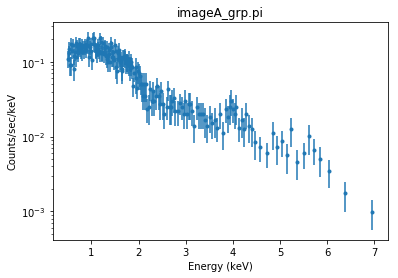
\includegraphics[width=0.5\textwidth]{pictures/imageA_grp}
	\caption{Example data taken from RXJ1131 OBSID 12833 Image A (Middle left)}
	\label{fig:exampleSherpa}
\end{figure}
\subsection{2D Plots}
We also can do some really nice 2D plots after running the following commands in the terminal:
\begin{lstlisting}
dmcopy "acisf12833_repro_evt2.fits[sky=region(simple.reg)]" source.fits
dmcopy "source.fits[events][bin x=::.1,y=::.1][IMAGE]" source_img.fits
\end{lstlisting}
Now with our source image created we can go about making 2D plots several ways using python...

\begin{lstlisting}
#OPTION A
import matplotlib
import matplotlib.pyplot as plt
%matplotlib inline
from astropy.io import fits
from matplotlib.colors import LogNorm
from astropy.wcs import WCS

image_file = "full_source_img.fits"
hdu_list = fits.open(image_file)
image_data = hdu_list[0].data
hdu_list.close()

hdu = fits.open(image_file)[0]
wcs = WCS(hdu.header)

plt.subplot(projection=wcs)
plt.imshow(image_data, cmap='jet', norm=LogNorm())
plt.colorbar()
plt.title(r'RX J1131-1231 Image A')
plt.xlabel('RA')
plt.ylabel('DEC')
\end{lstlisting}
\clearpage
\begin{figure}[h]
	\centering
	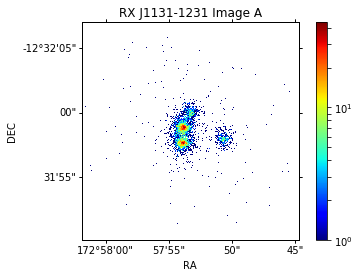
\includegraphics[width=0.5\textwidth]{pictures/optionA}
	\caption{Option A}
	\label{fig:2DopA}
\end{figure}

And after a little bit of fun with python coordinates:
\begin{lstlisting}
#OPTION B
import aplpy
from astropy.coordinates import SkyCoord
c1 = SkyCoord(ra=51.60*u.arcsec, dec=59*u.arcsec, distance=d_RXJ, frame='icrs') 
c2 = SkyCoord(ra=51.58*u.arcsec, dec=59*u.arcsec, distance=d_RXJ, frame='icrs') 
sep = c1.separation_3d(c2)  
fig = aplpy.FITSFigure(image_file)
fig.show_colorscale(cmap='jet')
fig.add_colorbar()
fig.colorbar.set_axis_label_text(r'Photon Flux $photons/cm^2/s$')
fig.add_scalebar(0.2*u.arcsec)
#fig.scalebar.set_length(0.02 * u.arcsecond)
fig.scalebar.set_color('white')
fig.scalebar.set_corner('top left')
fig.scalebar.set_label('%.2f Kpc' %(sep/u.kpc))
\end{lstlisting}
\begin{figure}[h]
	\centering
	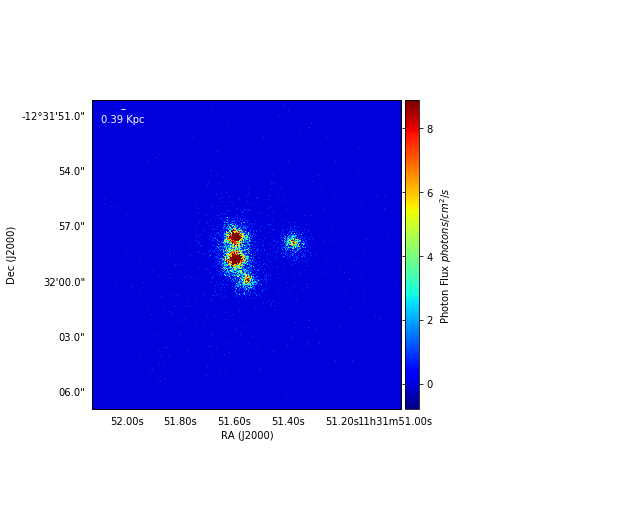
\includegraphics[width=0.7\textwidth]{pictures/optionB}
	\caption{Option B}
	\label{fig:2DopB}
\end{figure}
\clearpage
We also have the option of creating a true color image with the following bash script:
\begin{lstlisting}
#!/bin/bash

punlearn dmcopy 
pset dmcopy infile="full_source.fits[energy=200:1500][bin x=::.1,y=::.1]"
pset dmcopy outfile=soft_img.fits
pset dmcopy clobber=yes
dmcopy

punlearn dmcopy 
pset dmcopy infile="full_source.fits[energy=1500:2500][bin x=::.1,y=::.1]"
pset dmcopy outfile=med_img.fits
pset dmcopy clobber=yes
dmcopy

punlearn dmcopy 
pset dmcopy infile="full_source.fits[energy=2500:8000][bin x=::.1,y=::.1]"
pset dmcopy outfile=hard_img.fits
pset dmcopy clobber=yes
dmcopy

punlearn dmimg2jpg
pset dmimg2jpg infile=soft_img.fits
pset dmimg2jpg greenfile=med_img.fits
pset dmimg2jpg bluefile=hard_img.fits
pset dmimg2jpg outfile=truecolor.jpg
pset dmimg2jpg clobber=yes
dmimg2jpg
\end{lstlisting}
\begin{figure}[h]
	\centering
	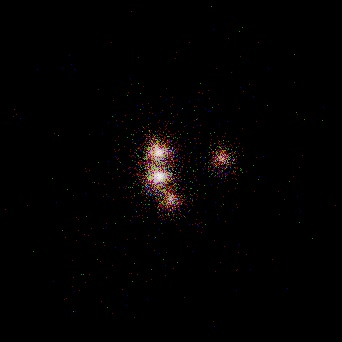
\includegraphics[width=0.5\textwidth]{pictures/trueColor}
	\caption{True Color}
	\label{fig:TC}
\end{figure}





\newpage
\section{Additional Python Fun}
\subsection{Lookback Time}
\begin{lstlisting}
from astropy import units as u
from astropy import cosmology
from astropy.coordinates import *
from astropy.cosmology import Planck13, default_cosmology
default_cosmology.set(Planck13)
z_RXJ = 0.658
d_RXJ = Distance(z=z_RXJ, unit=u.kpc)
\end{lstlisting}


\newpage

\section*{Bibliographies}
\bibliographystyle{plain}
\bibliography{bib.bib}
\end{document}